\section{Frog 3}
\subsection*{题意}
有$n$块石头(编号为 $1$到 $n$)排成一排,第 $i$块石头的高度为 $h_i$,并满足 $h_1 < h_2 < \cdots < h_N$。青蛙现在站在第 $1$ 块石头上。它可以从第 $i$ 块石头跳到第 $i + 1, i + 2, \ldots, N$ 块石头上。从第 $i$ 块石头跳到第 $j$ 块需要消耗 $(h_j - h_i)^2+C$ 点体力。请求出跳到第 $n$ 块石头所需的最小体力值。
\subsection*{数据范围}
\begin{itemize}
\item $2 \leq N \leq 2 \times 10^5$
\item $1 \leq C \leq 10^{12}$
\item $1 \leq h_1 < h_2 < \cdots < h_N \leq 10^6$
\end{itemize}

\subsection*{题解}
这题用到的技巧被称为\textbf{决策单调性}。这是一个貌似高端,但本质简单的知识点。下面我来分别介绍一下什么是\textbf{决策}和\textbf{单调性}。

\paragraph{什么是决策}首先,我们依旧设 $\texttt{dp[i]}$ 为跳到第 $i$ 块石头上所需的最小体力值。其次,用 $\texttt{cost}(i,k)$ 表示从 $i$ 转移到 $k$ 得到的值,表达式为 $\texttt{dp[i]} + (h_k - h_i)^2+C$。显然有 $\texttt{dp[k]} = \min\{\texttt{cost}(i,k) \mid 1\le i<k\}$。在计算$\texttt{dp[k]}$的时候,每一个转移源头$i$被称为一个\textbf{决策}。

枚举所有的决策的总复杂度是$O(n^2)$。这显然是不可承受的,于是我们需要探索更多性质。

\begin{center}
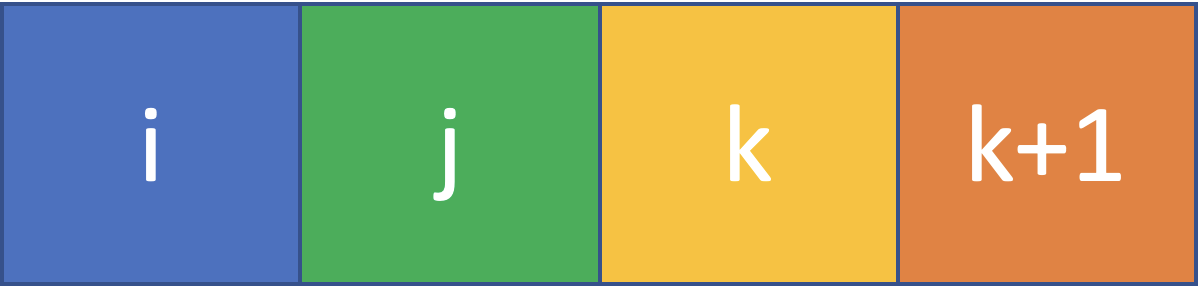
\includegraphics[width=3cm]{IJK.png}
\end{center}

\paragraph{什么是单调性}假设在考虑$\texttt{dp[k]}$的时候,决策$j$ 要优于决策$i$,即$\texttt{cost}(i,k) > \texttt{cost}(j,k)$,我们看看可以为计算 $\texttt{dp[k+1]}$ 提供什么便利。根据$\texttt{cost}(i,k)$的定义,我们可以得到决策$i$的成本增幅为:
\begin{equation*} 
\begin{split}
    \Delta_i 
    &= \texttt{cost}(i,k+1) - \texttt{cost}(i,k) \\
    &= \underbrace{(\texttt{dp[i]} + (h_{k+1} - h_i)^2+C)}_{\texttt{cost}(i,k+1)} - \underbrace{(\texttt{dp[i]} + (h_k - h_i)^2+C)}_{\texttt{cost}(i,k)}\\
    &= (h_{k+1} - h_i)^2 - (h_k - h_i)^2\\
    &= (h_{k+1} + h_k - 2h_i)(h_{k+1} - h_k) \ \textbf{(平方差公式)}\\
\end{split}
\end{equation*}
同理可得 $ \Delta_j   = (h_{k+1} + h_k - 2h_j)(h_{k+1} - h_k)$

注意到$h_i < h_j < h_k < h_{k+1}$是\textbf{单调递增}的,不难计算 $\Delta_i -  \Delta_j  = (2h_j-2h_i)(h_{k+1} - h_k) > 0$,即决策$i$的成本上升得比决策$j$更多。由于决策$j$本来就是更优的决策,它将一直保持优势下去。于是我们可以得出结论:\textbf{一旦一个决策被后来者打败,那么再也不需要被考虑}。

在计算一个状态的值的时候,我们定义成本最小的决策为最优决策,如有多种取最左的。举个例子:
\begin{center}
\begin{tabular}{ |c|c|c|c|c|c| } 
 \hline
 i & 1 &2 &3& 4& 5\\
 \hline
 最优决策 & N/A &1 &1& 2& 3\\
 \hline
\end{tabular}
\end{center}

由于之前的结论,最优决策从左到右一定是单调不下降的:只有可能出现 $\color{Red}{111}\color{Blue}{222}\color{YellowOrange}{333}$,而不会有$\color{Red}{111}\color{YellowOrange}{333}\color{Blue}{222}$。因为一旦 $\color{Blue}{2}$ 被 $\color{YellowOrange}{3}$ 打败,就永远不会比 $\color{YellowOrange}{3}$ 更优了。这就是所谓的\textbf{单调性}。

由于决策具有单调性,我们只需要二分出每个决策作为最优决策的起点即可。我们这里用\mintinline{cpp}{pair<int,int>}的数组实现,每个元素\mintinline{cpp}{(i,pos)} 表示决策 \mintinline{cpp}{i} 从 \mintinline{cpp}{pos}。开始成为最优策略。例如我们用 \mintinline{cpp}{[(1,1),(2,4),(3,7)]} 表示$\color{Red}{111}\color{Blue}{222}\color{YellowOrange}{333}$。


鉴于文字描述会过于冗长,直接观察以下伪代码:
\subsection*{核心代码}
\inputminted[linenos,autogobble]{python}{../Code/Z2.py}

\newpage